\documentclass{article}

\usepackage[title]{appendix}
\usepackage{bera} % not sure I love this font for this document
\usepackage{cite}
\usepackage{caption}
\usepackage[letterpaper,top=2cm,bottom=2cm,left=3cm,right=3cm,marginparwidth=1.75cm]{geometry}
\usepackage{graphicx}
\usepackage[colorlinks=true, allcolors=blue]{hyperref}
\usepackage{listings}
\usepackage{subcaption}
\usepackage{wrapfig}
\usepackage{xcolor}

\lstset{
    basicstyle=\bfseries\ttfamily,
    breaklines=true
}

\colorlet{punct}{red!60!black}
\definecolor{background}{HTML}{EEEEEE}
\definecolor{delim}{RGB}{20,105,176}
\colorlet{numb}{magenta!60!black}

\lstdefinelanguage{json}{
    basicstyle=\normalfont\ttfamily,
    numbers=left,
    numberstyle=\scriptsize,
    stepnumber=1,
    numbersep=8pt,
    showstringspaces=false,
    breaklines=true,
    frame=lines,
    backgroundcolor=\color{background},
    literate=
     *{0}{{{\color{numb}0}}}{1}
      {1}{{{\color{numb}1}}}{1}
      {2}{{{\color{numb}2}}}{1}
      {3}{{{\color{numb}3}}}{1}
      {4}{{{\color{numb}4}}}{1}
      {5}{{{\color{numb}5}}}{1}
      {6}{{{\color{numb}6}}}{1}
      {7}{{{\color{numb}7}}}{1}
      {8}{{{\color{numb}8}}}{1}
      {9}{{{\color{numb}9}}}{1}
      {:}{{{\color{punct}{:}}}}{1}
      {,}{{{\color{punct}{,}}}}{1}
      {\{}{{{\color{delim}{\{}}}}{1}
      {\}}{{{\color{delim}{\}}}}}{1}
      {[}{{{\color{delim}{[}}}}{1}
      {]}{{{\color{delim}{]}}}}{1},
}

\definecolor{lightgray}{rgb}{.9,.9,.9}
\definecolor{darkgray}{rgb}{.4,.4,.4}
\definecolor{purple}{rgb}{0.65, 0.12, 0.82}
\lstdefinelanguage{OldTypeScript}{
  keywords={abstract, any, as, boolean, break, case, catch, class, console, const, continue, debugger, declare, default, delete, do, else, enum, export, extends, false, finally, for, from, function, get, if, implements, import, in, infer, instanceof, interface, keyof, let, module, namespace, never, new, null, number, object, package, private, protected, public, readonly, require, return, set, static, string, super, switch, symbol, this, throw, true, try, type, typeof, undefined, unique, unknown, var, void, while, with, yield},
  morecomment=[l]{//},
  morecomment=[s]{/*}{*/},
  morestring=[b]',
  morestring=[b]",
  ndkeywords={class, export, boolean, throw, implements, import, this},
  keywordstyle=\color{blue}\bfseries,
  ndkeywordstyle=\color{darkgray}\bfseries,
  identifierstyle=\color{black},
  commentstyle=\color{purple}\ttfamily,
  stringstyle=\color{red}\ttfamily,
  sensitive=true,
  backgroundcolor=\color{lightgray},
  extendedchars=true,
  basicstyle=\ttfamily,
  showstringspaces=false,
  showspaces=false,
  numbers=left,
  numberstyle=,
  numbersep=9pt,
  tabsize=2,
  breaklines=true,
  showtabs=false,
  captionpos=b
}

\colorlet{comment}{green}
\lstdefinelanguage{TypeScript}{
    basicstyle=\normalfont\ttfamily,
    numbers=left,
    numberstyle=\scriptsize,
    stepnumber=1,
    numbersep=8pt,
    showstringspaces=false,
    breaklines=true,
    frame=lines,
    backgroundcolor=\color{background},
    literate=
     *{0}{{{\color{numb}0}}}{1}
      {1}{{{\color{numb}1}}}{1}
      {2}{{{\color{numb}2}}}{1}
      {3}{{{\color{numb}3}}}{1}
      {4}{{{\color{numb}4}}}{1}
      {5}{{{\color{numb}5}}}{1}
      {6}{{{\color{numb}6}}}{1}
      {7}{{{\color{numb}7}}}{1}
      {8}{{{\color{numb}8}}}{1}
      {9}{{{\color{numb}9}}}{1}
      {:}{{{\color{punct}{:}}}}{1}
      {,}{{{\color{punct}{,}}}}{1}
      {\{}{{{\color{delim}{\{}}}}{1}
      {\}}{{{\color{delim}{\}}}}}{1}
      {[}{{{\color{delim}{[}}}}{1}
      {]}{{{\color{delim}{]}}}}{1},
    morecomment=[l]{//},
    morecomment=[s]{/*}{*/},
    commentstyle=\color{green}\ttfamily
}

\graphicspath{ {./images/} }

\title{Developing a Visual Studio Code Language Support Extension for the Snail Programming Language}
\author{Charles Reinhardt}

\begin{document}
\maketitle

\begin{abstract}

    A high quality programming environment (often an integrated development environment, or IDE) can be vital to enhancing developer productivity. Visual Studio Code (VS Code) is a popular, open-source text editor maintained by Microsoft. VS Code delivers language-specific features through freely dowloadable, community-built extensions on an online marketplace. Many of these extensions allow developers to take advantage of editing features such as syntax highlighting, code-autocompletion, or debugging support. The snail language (Strings Numbers Arrays and Inheritance Language) is a simple, object-oriented programming langauge meant to be implemented in a one-semester undergraduate course. We present a new VS Code extension to provide language support for the snail language. The extension implements support for syntax highlighting, rudimentary auto-completion, and static error-checking diagnostics using VS Code's Langauge Server Protocol. This report summarizes the contents of a VS Code extension and gives an overview of how an extension runs, particularly highlighting the functions of VS Code's Langauge Server Protocol. I also discuss how this extension can be futher developed to make use of VS Code's Debug Adapter Protocol to implement a debugger with breakpoints, start/stop behavior, and variable inspection.

\end{abstract}

\section{Introduction}

Much of software development in the present day takes place in integrated development environments (IDEs) \cite{JetBrains_2019}. An IDE is a collection of software development tools, such as a code editor, debugger, and build system, often unified under a similar user interface, with the goal of simplifying the software development process and enhancing developer productivity \cite{Gillis_Silverthorne_2018,Shyniaieva_2023}. In addition to composing these tools together, many IDEs also offer advanced features within their code editors such as syntax highlighting, code auto-completion, and error-checking diagnostics. Today, there are any number of different IDEs available for use with any given programming language, many offered as freely-downloadable for public use. For example, a developer looking to write code in Java may choose to do so in Eclipse, IntelliJ IDEA, or BlueJ \cite{EclipseFoundation_2023, JetBrains_2023,KingsProgrammingEducationToolsGroup_2022}. With so many high quality IDEs available today, it is no surprise that 75\% of software developers today use an IDE in their everyday work \cite{JetBrains_2019}. Clearly, the IDE has become an integral part of the software development process today \cite{Vaniukov_2023}. 

Visual Studio Code (VS Code), is a popular, open source text editor maintained by Microsoft \cite{StackOverflow_2022,Microsoft_2023a}. When first downloaded, VS Code is a lightweight text editor with minimal features. However, a number of community-built, freely downloadable extensions offer advanced langauge features. These extensions can be dowloaded on VS Code's online extension marketplace, and can turn VS Code into a very fast ,robust, and powerful development environment for any programming task or language \cite{Microsoft_2023b}. 

The snail programming language (Strings Numbers Arrays and Inheritance Language) is a simple, object-oriented programming language meant to be implemented in a one-semester undergraduate course \cite{Angstadt_2023a}. In order to be implemented in a short time frame, snail is defined by limited features and a relatively annoying syntax. The language lacks a for-loop structure, opting instead to provide only while-loops. Each if statment \emph{requires} an else clause, even when the developer does not need to use one. Every statement must end with a semi-colon, which is not an issue until you accidentally forget one, and the resulting parse error message is wildly uninformative. While this design makes snail easier to implement, it makes it hard for a developer to write programs in snail.

Currently, there are no tools to offer advanced langauge support for the snail language. This is no surprise, as snail has a small user base and was first released in February 2022 \cite{Angstadt_2023b}. With no external support for the language, software developers are taken out of their comfort zone and are offered no guidance when navigating the snail language.

This report presents the Snail Language Support VS Code extension, which seeks to address the lack of programming support tools for the snail programming language. Snail Langauge Support provides several important features to make programming in the snail language easier. First, it features syntax highlighting to make reading snail code easier and help highlight key structures or keywords of the language. Further, it features rudimentary auto completion with auto-closing brackets, braces, and quotes, as well as if-else, while loop, and class definition snippets, reducing the burden of memorizing snail's strict and unintuitive syntax. The extension also has automatic, real-time error checking diagnostics that allow a user to see syntax or parse errors in a snail program before running it for themselves. Finally, the extension is structured to support a full debugger with breakpoints, step-in, step-over, and step-out functionality. 

This paper will outline the process of building the Snail Language Support VS Code extension.\footnote{This paper is formatted using \LaTeX. Recognizing that using \LaTeX \hspace{1pt} is really hard, the \LaTeX \hspace{1pt} source code for this paper can be found hosted on GitHub: \url{https://github.com/CharlesReinhardt/snail-language-support-paper/}} Specificaly, we will introduce the structure of a VS Code extension that is meant to add support for new programming langauges. We will also discuss how this extension uses VS Code's language server protocol (LSP) to provide realtime error diagnostics \cite{Microsoft_2022a}. We will address how the Snail Language Support extension may be further developed to include debugging support with breakpoints, step in/out behavior, and variable inspection, particularly highlighting the role of VS Code's debug adapter protocol (DAP) \cite{Microsoft_2021a}. Finally, we will review good software development practices such as version control and documentation. 

\section{Background}

In this section, we will discuss the history of integrated development environments (IDEs) and debuggers, and how they both assist software developers today. We will also discuss Visual Studio Code (VS Code) in more detail, identifying the technologies that power VS Code. 

\subsection{History of the Modern Integrated Development Environment}

The first programming environment to remotely resemble a modern IDE was the Dartmouth BASIC programming language run on the Dartmouth Time Sharing System (DTSS), developed in the mid 1960s \cite{KemenyKurtz_1968, Kurtz_1978}. Dartmouth BASIC was an example of a compile and go system, where program compilation was not separated from program execution \cite{Weik_2001}. Additionally, the DTSS also placed focus on making sharing time on a single university computer a simpler task, in order to help make programming more accessible to novices. This makes the DTSS an early example of combining multiple software development tasks into a single programming environment.

Borland's TurboPascal takes this idea one step further. Released in 1983, TurboPascal featured a Pascal compiler, code editor, file navigation user interface, and a rudimentary debugger \cite{Gajic_2017, Intersimone_2010, Wadlow_1984}. This time period would also see language-specific IDEs in Microsoft's Visual BASIC 1.0, Microsoft's QuickC, and Borland's Turbo C/C++, all featuring similar characteristics of early IDEs \cite{Burgwin_2013, Plant_Murrell_2007, Posch_2023, Forer_Petreley_1991}.

While early IDEs certainly had their merits, they usually only supported one programming language. Microsoft's Visual Studio, released in 1997, was one of the first IDEs to package support for a variety of programming languages in one piece of software \cite{Microsoft_1997}. Visual Studio also featured extensive tools to aid in development for software on the early internet. 
T
oday, we see a trend towards open source IDEs such as Eclipse, NetBeans, or VS Code \cite{Apache_2023, EclipseFoundation_2023, Microsoft_2023a}. Even open source editors such as these include advanced development features such as an intelligent code editor, debugging tools, and version control integration. Many of these editors have advanced features within their code editors, providing functions such syntax highlighting, code autocompletion, and realtime error diagnostics. 

There are many benefits to developing software using modern IDEs. By bundling code editing, build systems, and program execution into one tool, modern IDEs reduce the time and effort a developer needs to put forth in order to test a piece of code \cite{Gillis_Silverthorne_2018}. This also reduces the number of decisions a developer has to make while developing code, which can help increase productivity. Using an IDE can also standardize the software development process, by either helping a group of people use a consistent UI (and know how to help eachother), or allow a developer to avoid switching applications to complete a single task \cite{Veracode_2020}. 

\subsection{History of Modern Debugging Tools}

Debugging is the process of searching for and fixing unexpected errors in a piece of code \cite{AWS_2023}. Early techniques of debugging software involved physically printing machine output and reading, step-by-step, through code and output, searching for a potential error \cite{RevDeBug_2020}. Some computer systems, such as the IBM 704 Data Processing system released in 2968, allowed programmers to print information stored in specified memory locations in specified forms to assist with debugging activities \cite{MIT_1957, IBMArchives_2023}. 

The \lstinline{adb} and \lstinline{dbx} debuggers for the Unix operating system saw a release in the 1970s and 1980s \cite{BellLaboratories_1983, Linton_1990}. These tols introduced the concept of breakpoints, which help a developer pinpoint the location of a fault in a piece of code. Both \lstinline{adb} and \lstinline{dbx} were run on the command line. Next, came the GNU project debugger (\lstinline{gdb}), another command line debugger, released in 1986, which gave the user even greater control of tracing a program's execution throughout its runtime \cite{GNU_FSF_2023}. With the ability to debug low-level languages like C and Assembly, \lstinline{gdb} is still in use today.

Modern debuggers with graphical user interfaces (GUIs) include the Visual Studio Debugger, which allows a developer to track variable values, function calls, and even change pieces of code or values of expressions while debugging \cite{Microsoft_2022b}. Eclipse, a popular IDE for Java, has a similar debugger with a user friendly GUI \cite{Sinha_2017}. Today, many developement workflows include the use of debugging tools \cite{Matloff_Salzman_2008}.

Debugging tools can be of great assistance to developers. By allowing developers to more closely and quickly inspect a program's execution, debugging tools can reduce the amount of time a developer spends debugging, and thus enhance developer productivity \cite{ZhRaAmRuWo_2008}. 

\subsection{What is Visual Studio Code?}

Visual Studio Code is a popular, open source code editor. Visual Studio Code is designed to be fast and lightweight, with a focus on allowing a developer to write, test, adn debug source code quickly \cite{Microsoft_2023c}. To achieve this, VS Code uses native, web, and language-specific technologoies. Tools like Electron allow VS Code to run on multiple platforms and operating systems using common web technologies like JavaScript, HTML, and CSS \cite{Electron_2023}.

While VS Code is lightweight and fast, it still supports advanced features such as build or debugger tools available through the online VS Code extension marketplace \cite{Microsoft_2023b}. VS Code is designed for extensibility, providing robust APIs to allow independent developers to create and publish extensions \cite{Microsoft_2023d}. As a result, VS Code is able to grow and develop along with its community of users. 

Existing extensions make VS Code a popular code editor \cite{StackOverflow_2022}. The CodeSnap extension allows a user to capture and share improved screenshots of code \cite{adpyke_2021}. GitLens adds additional visualization tools to help developers contribute to Git repositories while editing in VS Code \cite{GitKraken_2023}. Language Support for Java(TM) provides intellisense, formatting, refactoring, and build system support for the Java language \cite{RedHat_2023}. The result of this extension support is an IDE that is used by over 75\% of professional and hobby software developers \cite{StackOverflow_2022}. 

\section{Anatomy of a Visual Studio Code Extension}

In this section, we will discuss the contents of a Visual Studio Code (VS Code) extension. First, we will highlight the directory structure of a typical language support VS Code extension. Next, we will discuss how a VS Code extension runs, from the moment it starts up to the moment it shuts down. We will also overview what can be provided to the user by a VS Code extension, specifically highlighting language configurations, autocompletion, and syntax highlighting. 

\subsection{Directory Structure}

Most VS Code extensions share a similar directory structure. These structures may vary depending on what purpose the extension is meant to serve. In figure \ref{fig:directory-structure}, we see a diagram of a typical language support VS Code extension. First, the \lstinline{.vscode} directory configures how we run and test our exstension locally. Through the \lstinline{launch.json} and \lstinline{tasks.json} files, we define various tasks and configurations to streamline the build and testing process.\footnote{From personal experience, we strongly recommend taking the time to understand these files before developing a VS Code extension. It will likely save painstaking debugging in the near future. See launch configurations: \url{https://code.visualstudio.com/docs/editor/debugging\#_launch-configurations} and tasks: \url{https://code.visualstudio.com/docs/editor/tasks}} Note that these configuration files do not get packaged with a released VS Code extension. Next, a \lstinline{README.md} file allows us to advertise the features of our extension. This file is rendered in the VS Code extension marketplace and is meant to be a user's first impression of an extension.

Snail Langauge Support is built with TypeScript. TypeScript is a syntactic superset of JavaScript that allows the developer the benefits of a type system without sacrificing JavaScript's flexibility \cite{TypeScript_2023}. TypeScript files are denoted with a \lstinline{.ts} suffix. Using the TypeScript compiler (\lstinline{tsc}), a program in TypeScript is transpiled to an equivalent JavaScript program. With a \lstinline{tsconfig.json} file in an extension directory, we define how the TypeScript compiler handles an extension's TypeScript code. We define where the compiler looks for our \lstinline{.ts} files, where to place resulting JavaScript files, and the strictness of type checks during transpilation.


\begin{wrapfigure}{R}{0.3\textwidth}
    \begin{center}
        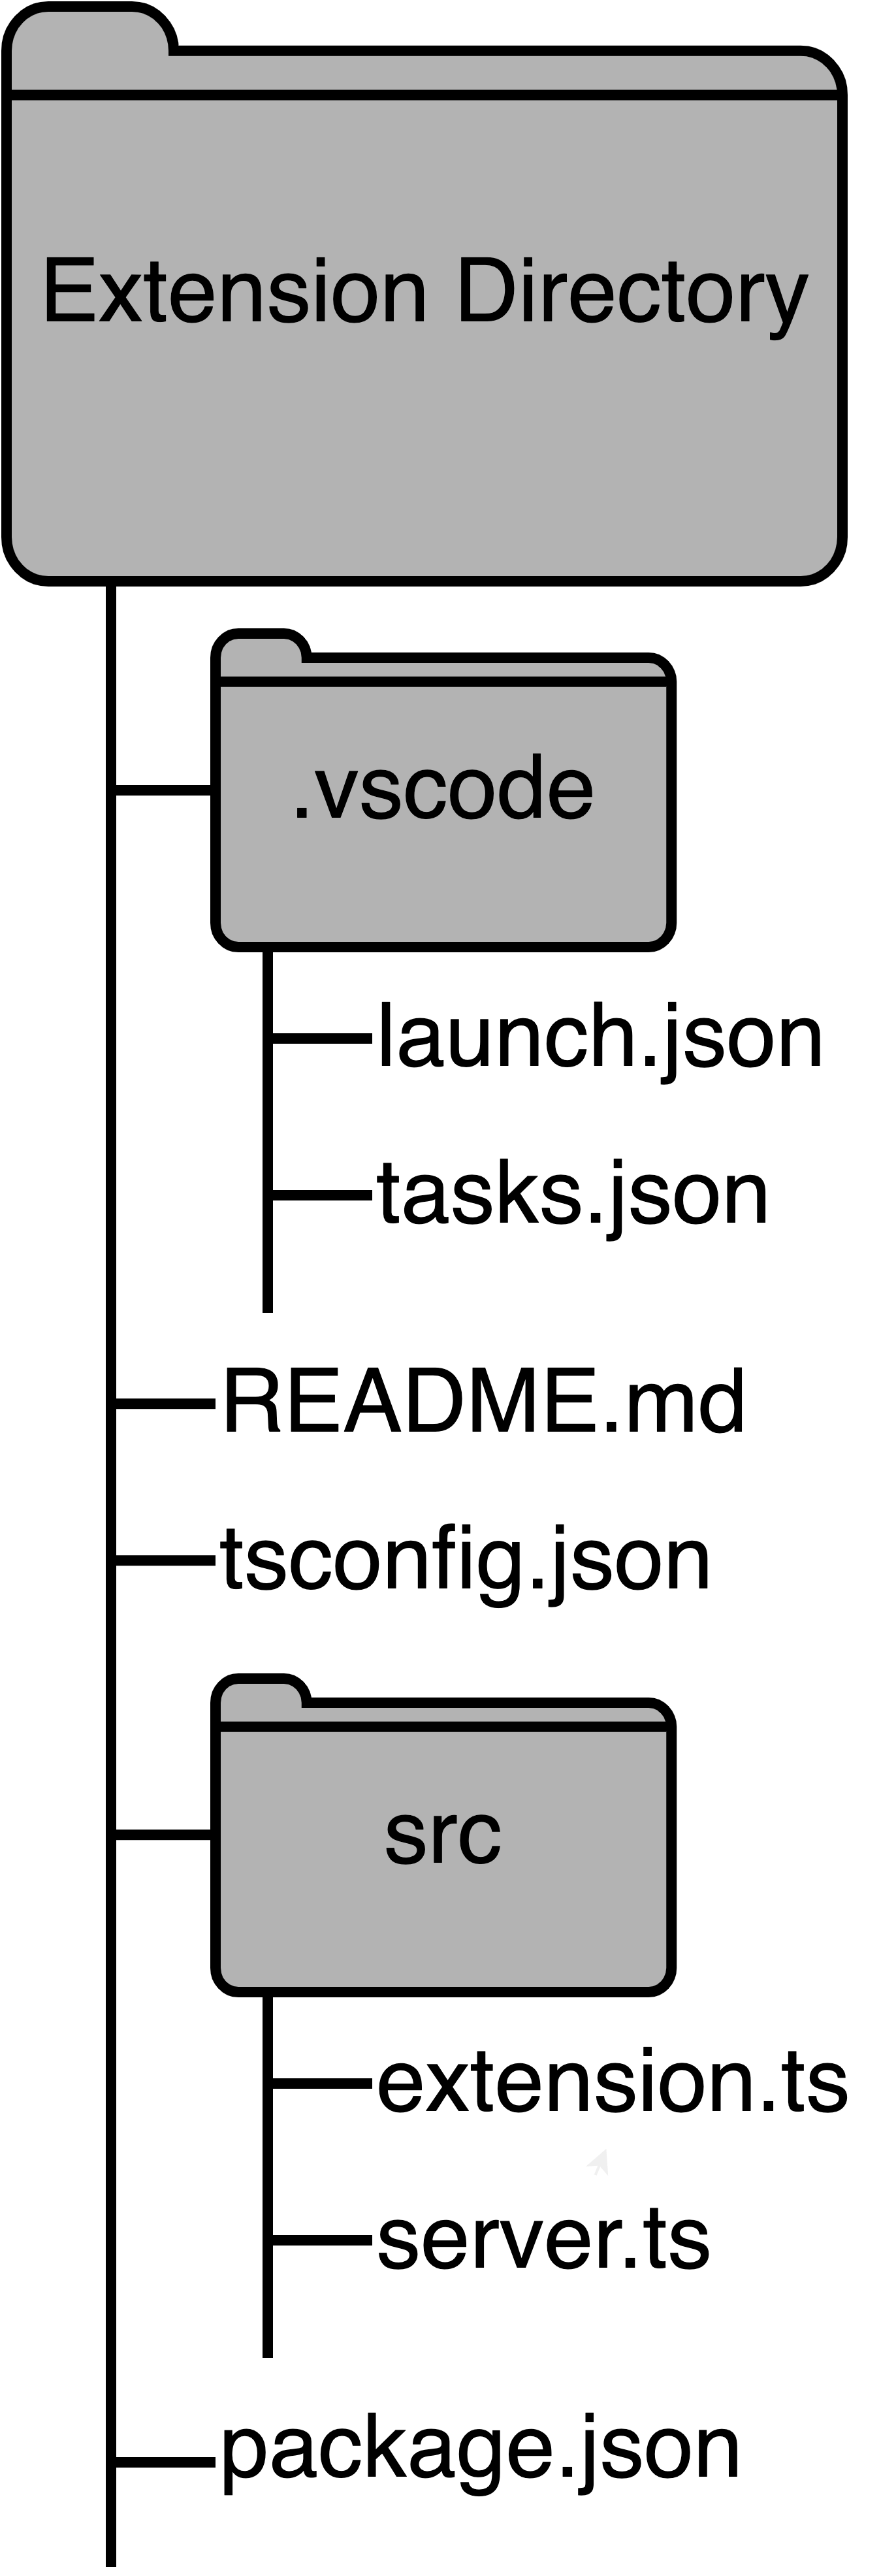
\includegraphics[height=0.3\textheight]{directory-structure.png}
        \caption{
            \centering 
                The typical directory structure of a VSCode language support extension.
        }
        \label{fig:directory-structure}
    \end{center}
\end{wrapfigure}

The \lstinline{src} directory contains the aforementioned TypeScript source code that runs our extension. In this directory, the \lstinline{extension.ts} file defines special actions for our extension and launches the extension within an existing VS Code window. The \lstinline{server.ts} file defines a language server that allows our extension to take advantage of realtime error diagnostics. We further discuss language servers later in this paper. 

Lastly, the \lstinline{package.json} file defines which features and configurations our extension supports. It also contains some biographical information about the extension, such as the author, publisher, or name of the exstension. 

To build the structure for Snail Language Support, we used the \lstinline{Yeoman} tool to generate an extension skeleton \cite{Yeoman_2023}. This skeleton was instrumental in providing basic configuration and source files to modify into the Snail Language Support extension.

\subsection{Extension Lifecycle: From Startup to Shutdown}

When a VS Code window launches, it also launches all extensions the user has downloaded and enabled by calling each extension's \lstinline{activate} function, defined in the extension's source code. In Snail Language Support's case, the \lstinline{activate} function is defined in the \lstinline{extension.ts} file. This file has access to the VS Code extension API, allowing a developer to define certain VS Code client UI updates \cite{Microsoft_2023d}. For example, Snail Language Support can display a VS Code UI style error message to the user if the user does not have a compatibale version of the snail language dowloaded. 

The \lstinline{activate} function is responsible for a few different behaviors. First, the \lstinline{activate} function registers a few command handlers to watch for commands input from a user. A command handler is an example of the observer design pattern, which allows a developer to address a variety of potential input events that are experienced during runtime \cite{GangOfFour_1995}. A developer can register an observer that listens for a particular event and executes a block of code once that event is detected. Snail Language Support defines a few command handlers to detect when a user chooses to run or debug a snail file. We will touch on the topic of debugging within Snail Language Support more later. 

The \lstinline{activate} function also launches a snail language server, which communicates with VS Code via VS Code's Language Server Protocol (LSP). We further discuss the topic of language servers later in this paper.

Once the extension setup inside the \lstinline{activate} function is complete, VS Code enables the extension within the workspace, allowing a developer to utilize the functions of an extension. Once the VS Code window is closed, or the extension is manually disabled, VS Code calls the \lstinline{deactivate} function, which shuts down any separate processes left over from the extension run.

To inspect Snail Language Support's \lstinline{extension.ts} file more closely, see appendix \ref{app:extension-ts}

\subsection{Extension Contributions: The Extension Manifest}

Recall that the \lstinline{package.json} defines what our extension contributes to the user. We now discuss some of those contributions here.

First, we can define some metadata about our extension, such as a name, author, description, and version. We can also define which version of the VS Code engine this extension expects. This ensures that an extension knows which VS Code APIs it has proper access to. For example, an extension that expects a VS Code version of \lstinline{1.7.0} won't be able to take advantage of an API released in \lstinline{1.8.0} \cite{Microsoft_2023e}. We can also define some categories that our extension falls under, helping our extension gain visibility on the online VS Code marketplace.

Next, and very importantly, we define where the source code is located for our extension. Through the \lstinline{main} attribute, we define the entry point for our extension. This is the file that contains the \lstinline{activate} function. For Snail Language Support, this is the \lstinline{/out/extension.js} file. Notice that this is the transpiled version of our \lstinline{src/extension.ts} file. For a more detailed look at Snail Language Support's \lstinline{package.json} file, see appendix \ref{app:package-json}.

\subsubsection{Language Configuration}

Snail Language Support also provides language configuration settings supported by a VS Code extension. These configurations are found in \lstinline{language-configuration.json} file. We can define what is considered a commend through the \lstinline{comments.lineComment} or \lstinline{comments.blockComment} attributes, which allows a user to comment lines using VS Code's comment shortcut. Similarly, we can also define auto-closing structures such as parentheses or brackets through the \lstinline{autoClosingPairs} attribute, which allows VS Code to automatically place closing parentheses or brackets. This is particularly useful for snail, as more opening parentheses or brackets require a closing partner. By defining \lstinline{autoClosingPairs}, a developer can expend less mental energy ensuring that each parenthesis and bracket has a closing pair, and more mental energy on developing code. The \lstinline{language-configuration.json} file for Snail Language Support can be found in appendix \ref{app:language-configuration}. For more attributes and configuration options, see the VS Code documentation on language configurations \cite{Microsoft_2023f}.

\subsubsection{Rudimentary Autocompletion Through Snippets}

Snail Language Support provides autocompletion suppport for common structures such as if-else clauses, while loops, and class definitions. This autocompletion is implemented through VS Code snippets. A snippet is a commonly used code structure that is defined by a \lstinline{prefix} (or a few options for a \lstinline{prefix}) and a \lstinline{body}. When a user types a snippet \lstinline{prefix}, they are given the option to replace the keyword with the \lstinline{body} of the snippet to complete the structure. Snippet bodies can also contain placeholders, which a user can visit in sequence while pressing their \lstinline{tab} button. For a full listing of the snippets that Snail Language Support provides, see appendix \ref{app:snippets-json}. Similarly, for more information on snippets in VS Code, see the documentation \cite{Microsoft_2023g}.

\subsubsection{Syntax Highlighting}

Snail Language Support also supports syntax highlighting for the snail language as shown in figure \ref{fig:syntax-highlight}. VS Code's syntax highlighting makes heavy use of TextMate language grammars. A generic language grammar is a set of rules that govern what constitutes a valid statement for a given programming language \cite{pgrandinetti_2019}. A TextMate grammar is a specific format for defining a language grammar \cite{MacroMates_2021a}. TextMate grammars define patterns that match special elements of a text document and assign scope names to these elements. For example, keywords of a particular language might be assigned the \lstinline{keyword.control} scope name. These patterns are defined with regular expressions. 

\begin{figure}[b]
    \begin{subfigure}[c][][c]{0.45\textwidth}
        \begin{center}
            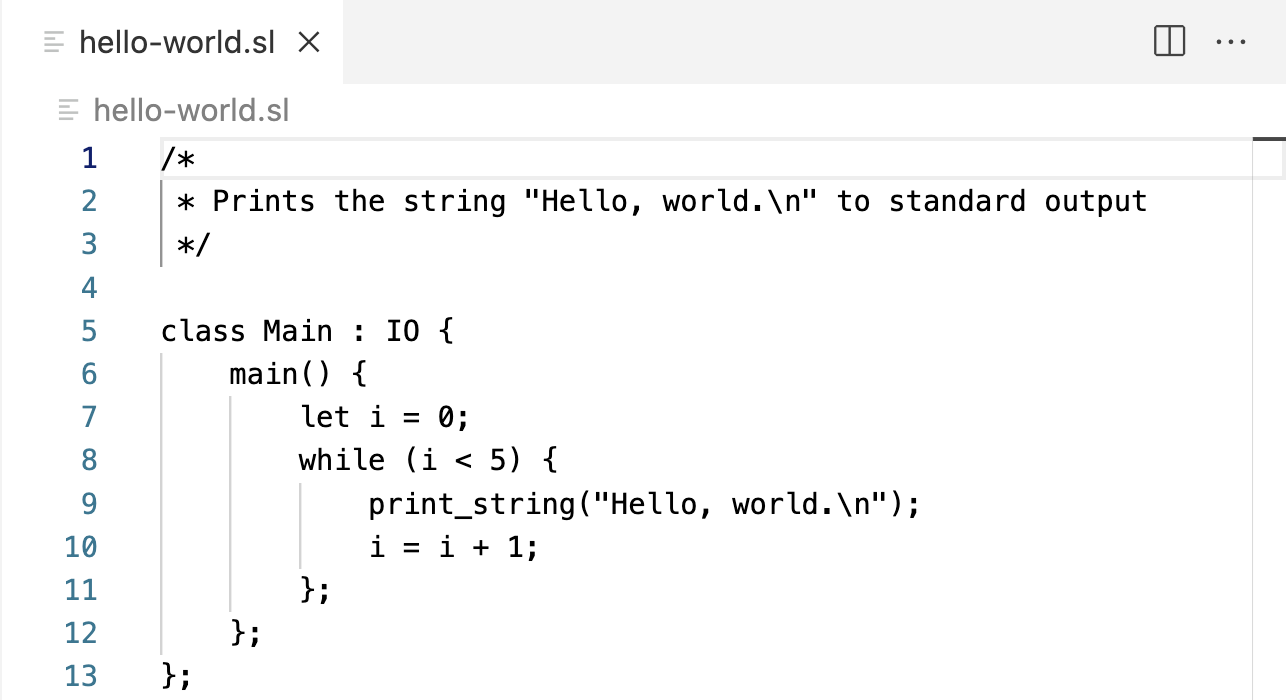
\includegraphics[width=\textwidth]{dev-no-highlight-light.png}
            \caption{Developing snail code without syntax highlighting can be a mentally taxing experience.}
            \label{fig:dev-no-highlight}
        \end{center}
    \end{subfigure}
    \hspace{0.05\textwidth}
    \begin{subfigure}[c][][c]{0.45\textwidth}
        \begin{center}
            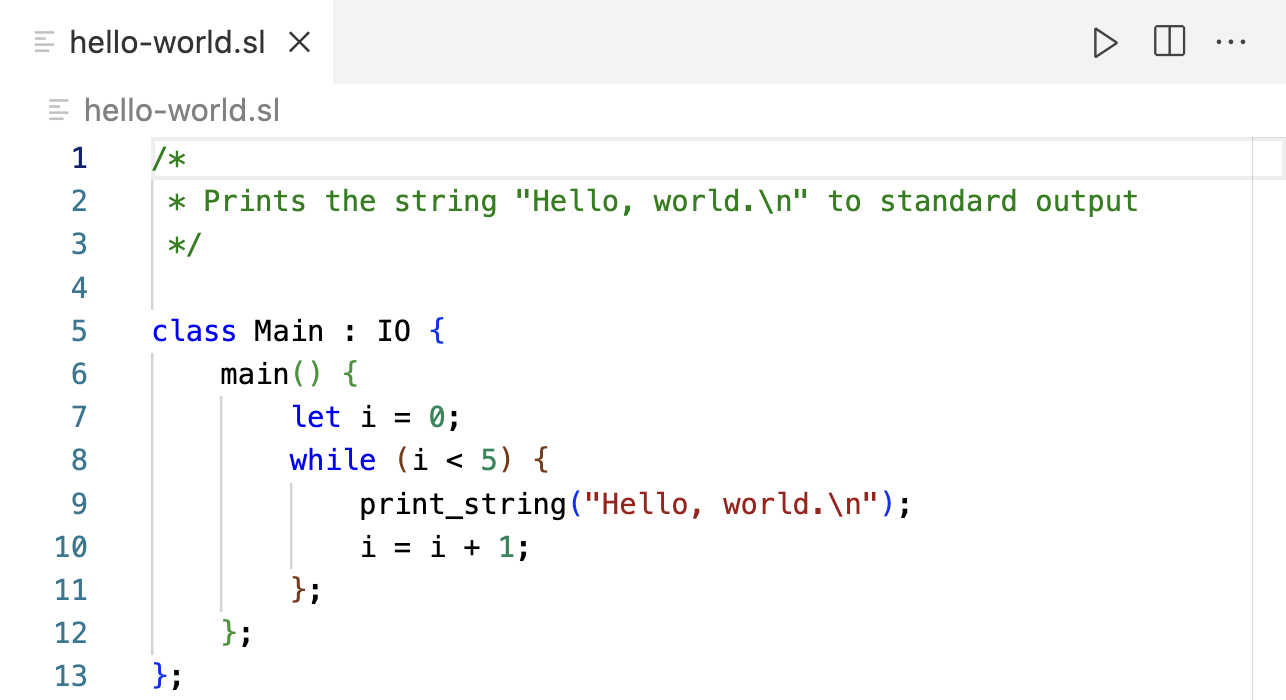
\includegraphics[width=\textwidth]{dev-with-highlight-light.png}
            \caption{Syntax highlighting makes developing snail code much easier.}
            \label{fig:dev-with-highlight}
        \end{center}
    \end{subfigure}
    \caption{Demonatrating the benefit of Snail Language Support's syntax highlighting feature.}
    \label{fig:syntax-highlight}
\end{figure}

A regular expression is a string of text that can be used to match a particular pattern in a piece of text. Regular expressions are used in a variety of programming activities, such as lexing a program or to find text in a code editor \cite{ComputerHope_2022, Cornell_2022}. 

TextMate grammars make use of the advanced Oniguruma regular expression syntax, developed by K. Kosako \cite{Microsoft_2023h, MacroMates_2021b}. The Oniguruma regular expression syntax offers advanced features such as case insentivity options, character groupings, quantifiers, and anchors. 

Snail Language Support defines a TextMate grammar in the \lstinline{snail.tmLanguage.json} file, shown in appendix \ref{app:snail-tmLanguage}. Taking a closer look at the structure of this document, we see three main relevant attributes: \lstinline{$schema}, \lstinline{patterns}, and \lstinline{repository}. 

First, the \lstinline{$schema} attribute links to a TextMate grammar schema document. This allows our editor to verify our \lstinline{snail.tmLanguage.json} file and ensure we are defining valid attributes.

Next, we define a series of \lstinline{patterns} using regular expressions.  VS Code's tokenization engine reads our snail file one line at a time and tries to match the text to a pattern (or combination of patterns) defined in our \lstinline{patterns} attribute. If the engine is successful in matching snail text to a pattern, it assigns that text a scope name. VS Code then uses these scope names to highlight the text appropriately, depending on the chosen color theme. 

The engine tries matching text in the order we define our patterns. This means that the first pattern we define in \lstinline{patterns} is the first regular expression that the tokenization engine tries to match to a line in a snail file. It is important to pay attention to the order that patterns are defined. For example, Snail Language Support defines comments first, which ensures that all snail text, no matter how complicated or syntactically complex, is highlighted as a simple comment.\footnote{While defining our regular expression patterns, we found the Rubular program essesntial. It allowed us to iterate and test regular expressions more rapidly. We strongly recommend investigating this site while developing a TextMate grammar of your own: \url{https://rubular.com/}} 

TextMate grammars also allow you to nest patterns inside of one another. This is essential for snail, as it allows the tokenization engine to match text inside of parentheses or brackets. TextMate grammars' ability to recursively reference the grammar itself (through the \lstinline{$self} keyword) is also essential for this functioanlity. 

For Snail Language Support, we define our patterns in the \lstinline{repository} attribute. This allows us to reference them in multiple places in our \lstinline{patterns} attribute. We feel this makes the document easier to understand and modify when necessary. 

It is important that Snail Language Support's syntax highlighting can handle a snail file with incorrect syntax. For example, if a snail file uses a class definition with the incorrect syntax, Snail Language Support should still be able to highlight the code contained in that class. To achieve this, we must make sure that all patterns are accessible from the top level of the grammar. While any pattern may be nested inside of another pattern, that pattern must be present elsewhere in the grammar so that it is not \emph{only} accessible after matching the other pattern.

\section{Language Servers and the Language Server Protocol (LSP)}

Snail Language Support also provides realtime lexing and parsing error diagnostics when developing code in snail. To do this, Snail Language Support uses a language server that communicates via VS Code's langauge server protocol (LSP). We now discuss what a language server is, how it relates to the LSP, and how Snail Language Support uses langauge servers. 

\subsection{What is a Language Server?}

\begin{wrapfigure}{r}{0.5\textwidth}
    \begin{center}
        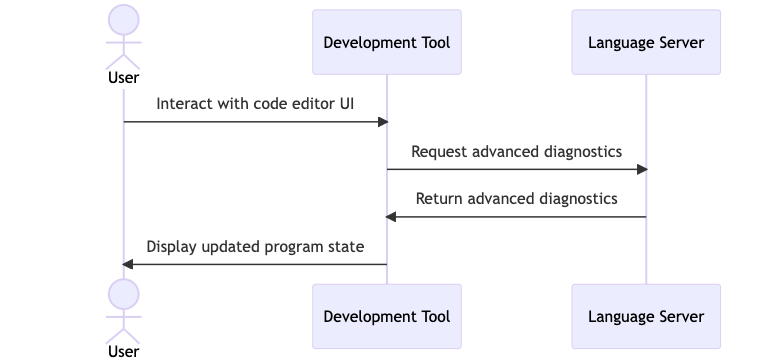
\includegraphics[width=0.5\textwidth]{language-server.png}
        \caption{
            \centering 
            A development tool will communicate with a language server to display advanced diagnostics.
        }
        \label{fig:language-server}
    \end{center}
\end{wrapfigure}

A language server is a tool used to provide language-specific editing features such as advanced autocomplete, go-to definition, or automatic error checking \cite{Microsoft_2022a}. Many IDEs today utilize language servers by launching a language server process that runs in the background while a developer writes code. The development tool then sends a \emph{requests} to the language server for, and the language server \emph{responds} with the information requested by the development tool. The development tool then displays the information to the developer. This process is displayed in figure \ref{fig:language-server}.

Many language servers are implemented in the language they assist with \cite{Microsoft_2023j}. For example, a typical Python language server would be implemented in Python. This makes integrating language servers into development tools difficult, as many development tools are written in languages other than the language they are meant to develop. Further, a single language server might have to interact with a number of different development tools. For example, a Python language server might have to interact with VS Code, PyCharm, and Spyder. Without a standard framework for communication between development tools and language servers, development tools and language servers must implement specific functionality for each pairing. This problem is displayed in figure \ref{fig:no-lsp-theory}. 

Each development tool has different standards for how they interact with language servers. To address this, a development tool may need to adjust how they request and recieve information from each language server it interacts with. Alternatively, a language server might adjust how it recieves and responds to requests for each development tool it interacts with. Both options are not ideal.

\subsection{The Language Server Protocol} 

The Langauge Server Protocol (LSP) defines a standard framework for development tool and language server communication \cite{Microsoft_2022a}. A development tool is able to communicate with any language-specific language server by sending requests and recieving responses according to the LSP standard. 

The LSP defines a number of common interactions between a development tool and a langauge server. For example, a development tool might send the \lstinline{DidchangeTextDocument} notification when a development tool detects that a text document has been edited. A language server might validate this text document and send any notable diagnostics back to the development tool. 

VS Code's LSP relies on requests and responses \cite{Microsoft_2023i}. A request is a message that a development tool sends to a language server, asking the language server to perform some operation. A language server responds to the request by sending a corresponding response message with information about the executed operation. In order to follow the LSP, a language server \textbf{must} send a corresponding response upon recieving any requests. For example, a development tool might send the \lstinline{Initialize} request to a language server, and a language server must respond with the \lstinline{InitializeResponse} before the development tool is allowed to send any further requests. This contract goes both ways: when a language server sends a request to a developement tool, the development tool must respond.

VS Code's LSP also uses notifications. A notification is a message that does not require a response. A development tool can send a notification to a language server and the language server can process the notification as it sees fit. Often, the language server will send information back to the development tool (in the form of another notification), but it is important to note that the language server is not required to respond. 

With an established standard for communication as shown in \ref{fig:lsp-theory}, both development tools and language servers can streamline their communications systems. Additionally, a developer producing one of these tools or features can rely on a consistent standard to make the development process easier. 

\begin{figure}
    \begin{subfigure}[c][][c]{0.45\textwidth}
        \begin{center}
            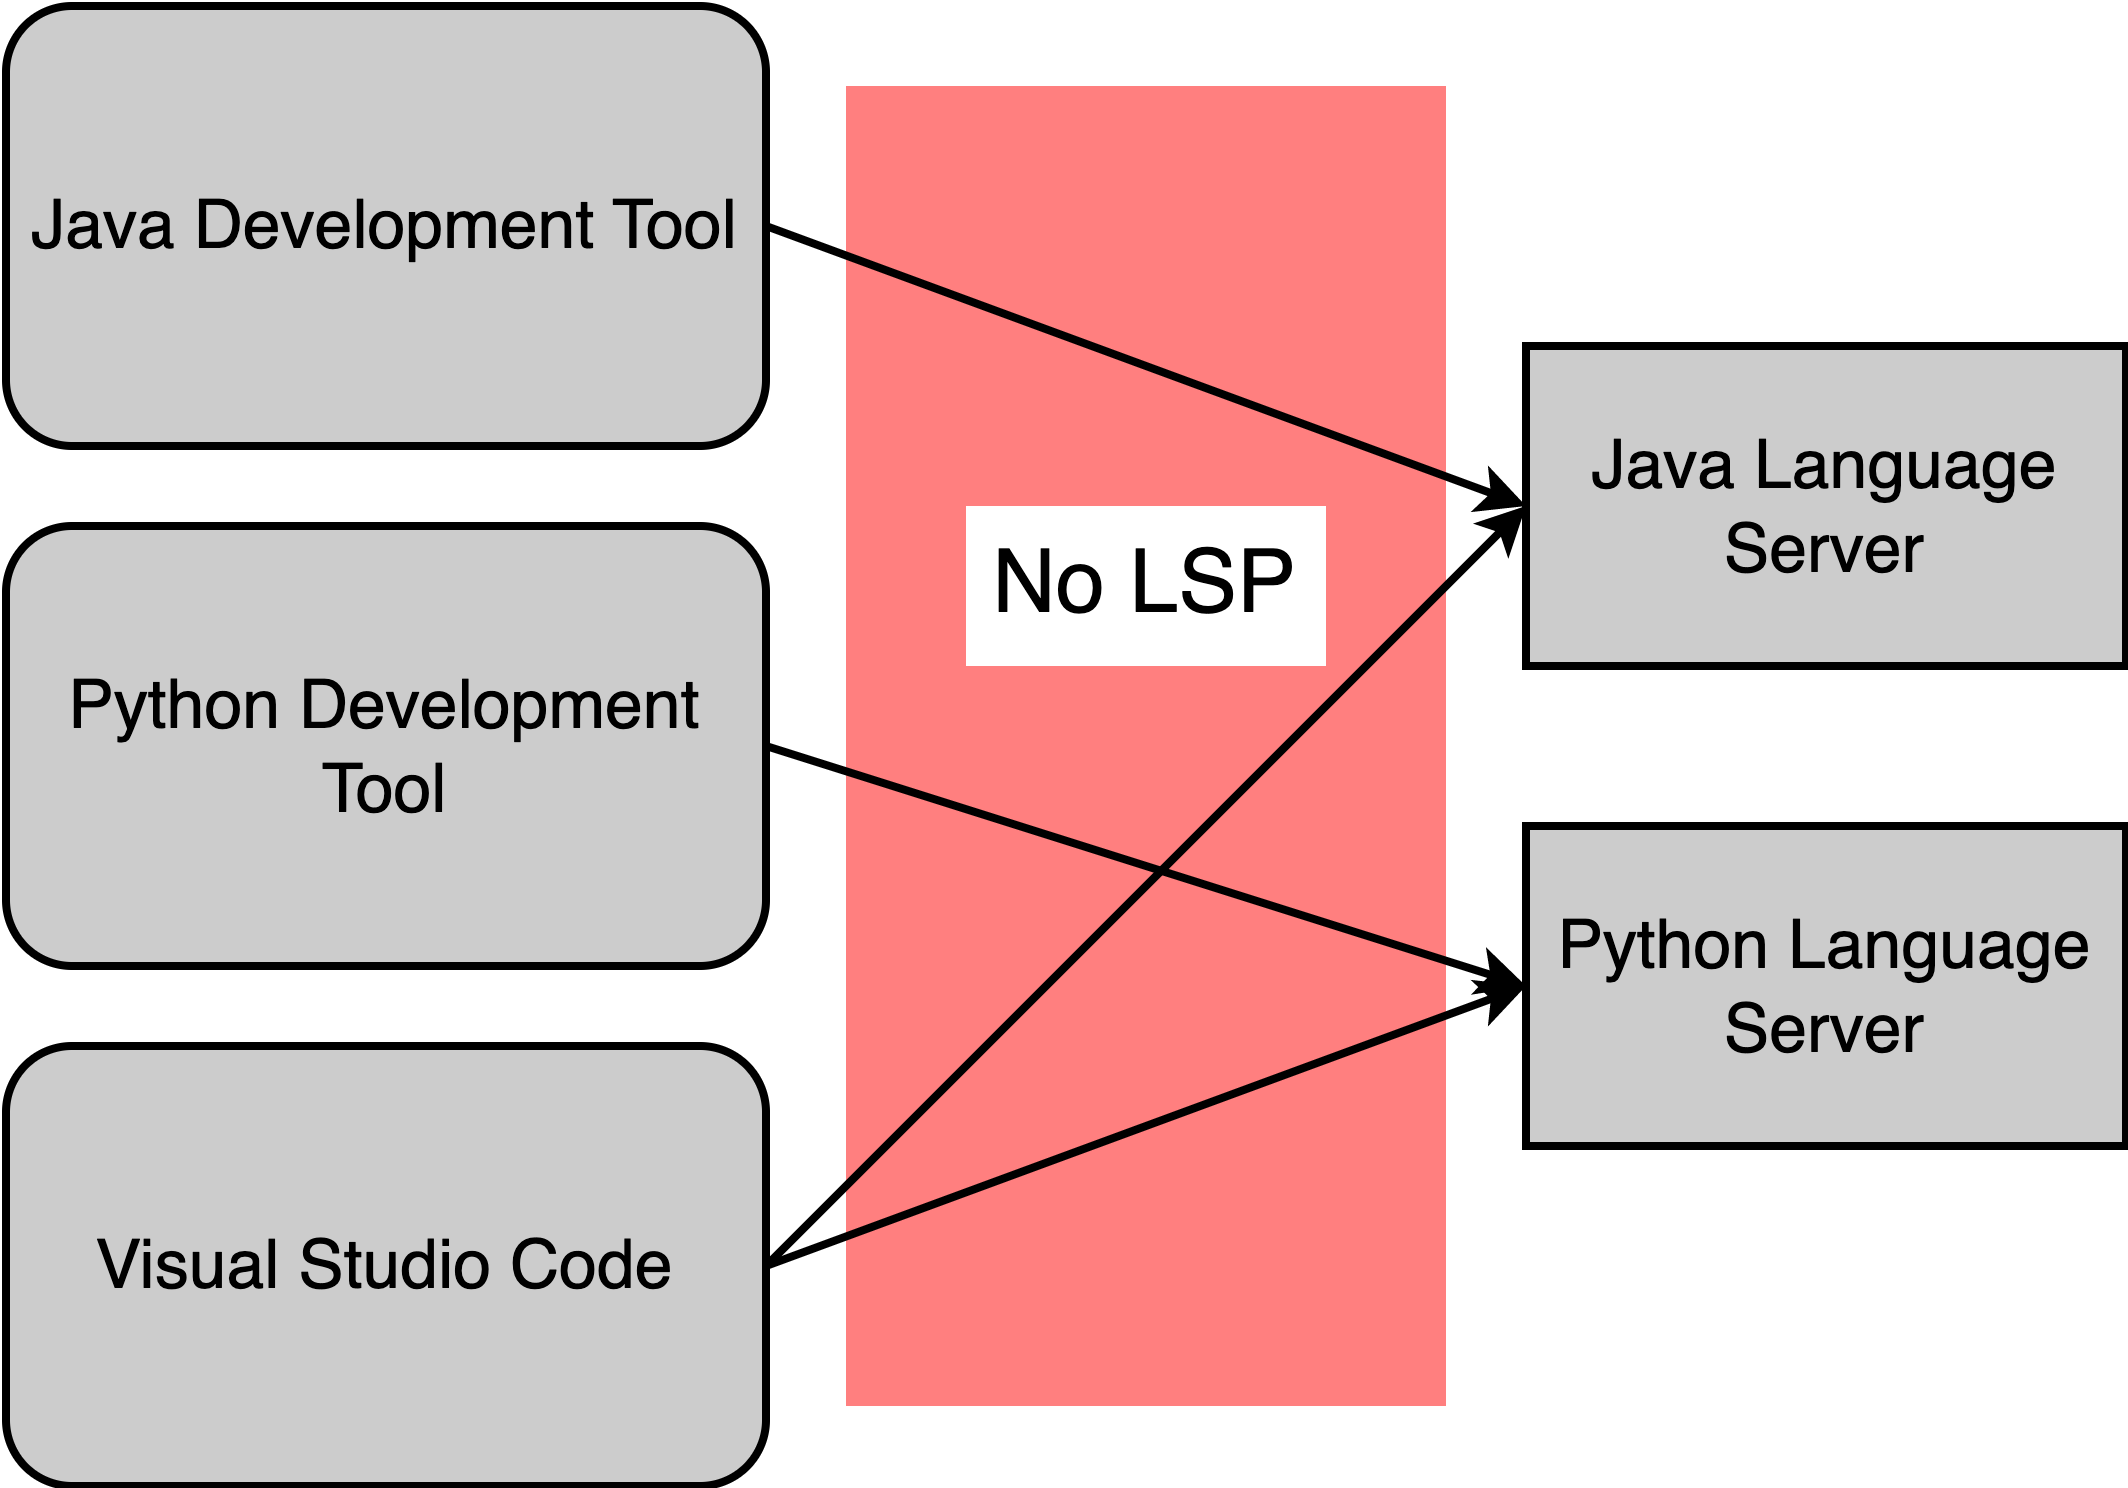
\includegraphics[width=\textwidth]{no-lsp-theory.png}
            \caption{Without the Language Server Protocol, development tool and language server communication can get messy.}
            \label{fig:no-lsp-theory}
        \end{center}
    \end{subfigure}
    \hspace{0.05\textwidth}
    \begin{subfigure}[c][][c]{0.45\textwidth}
        \begin{center}
            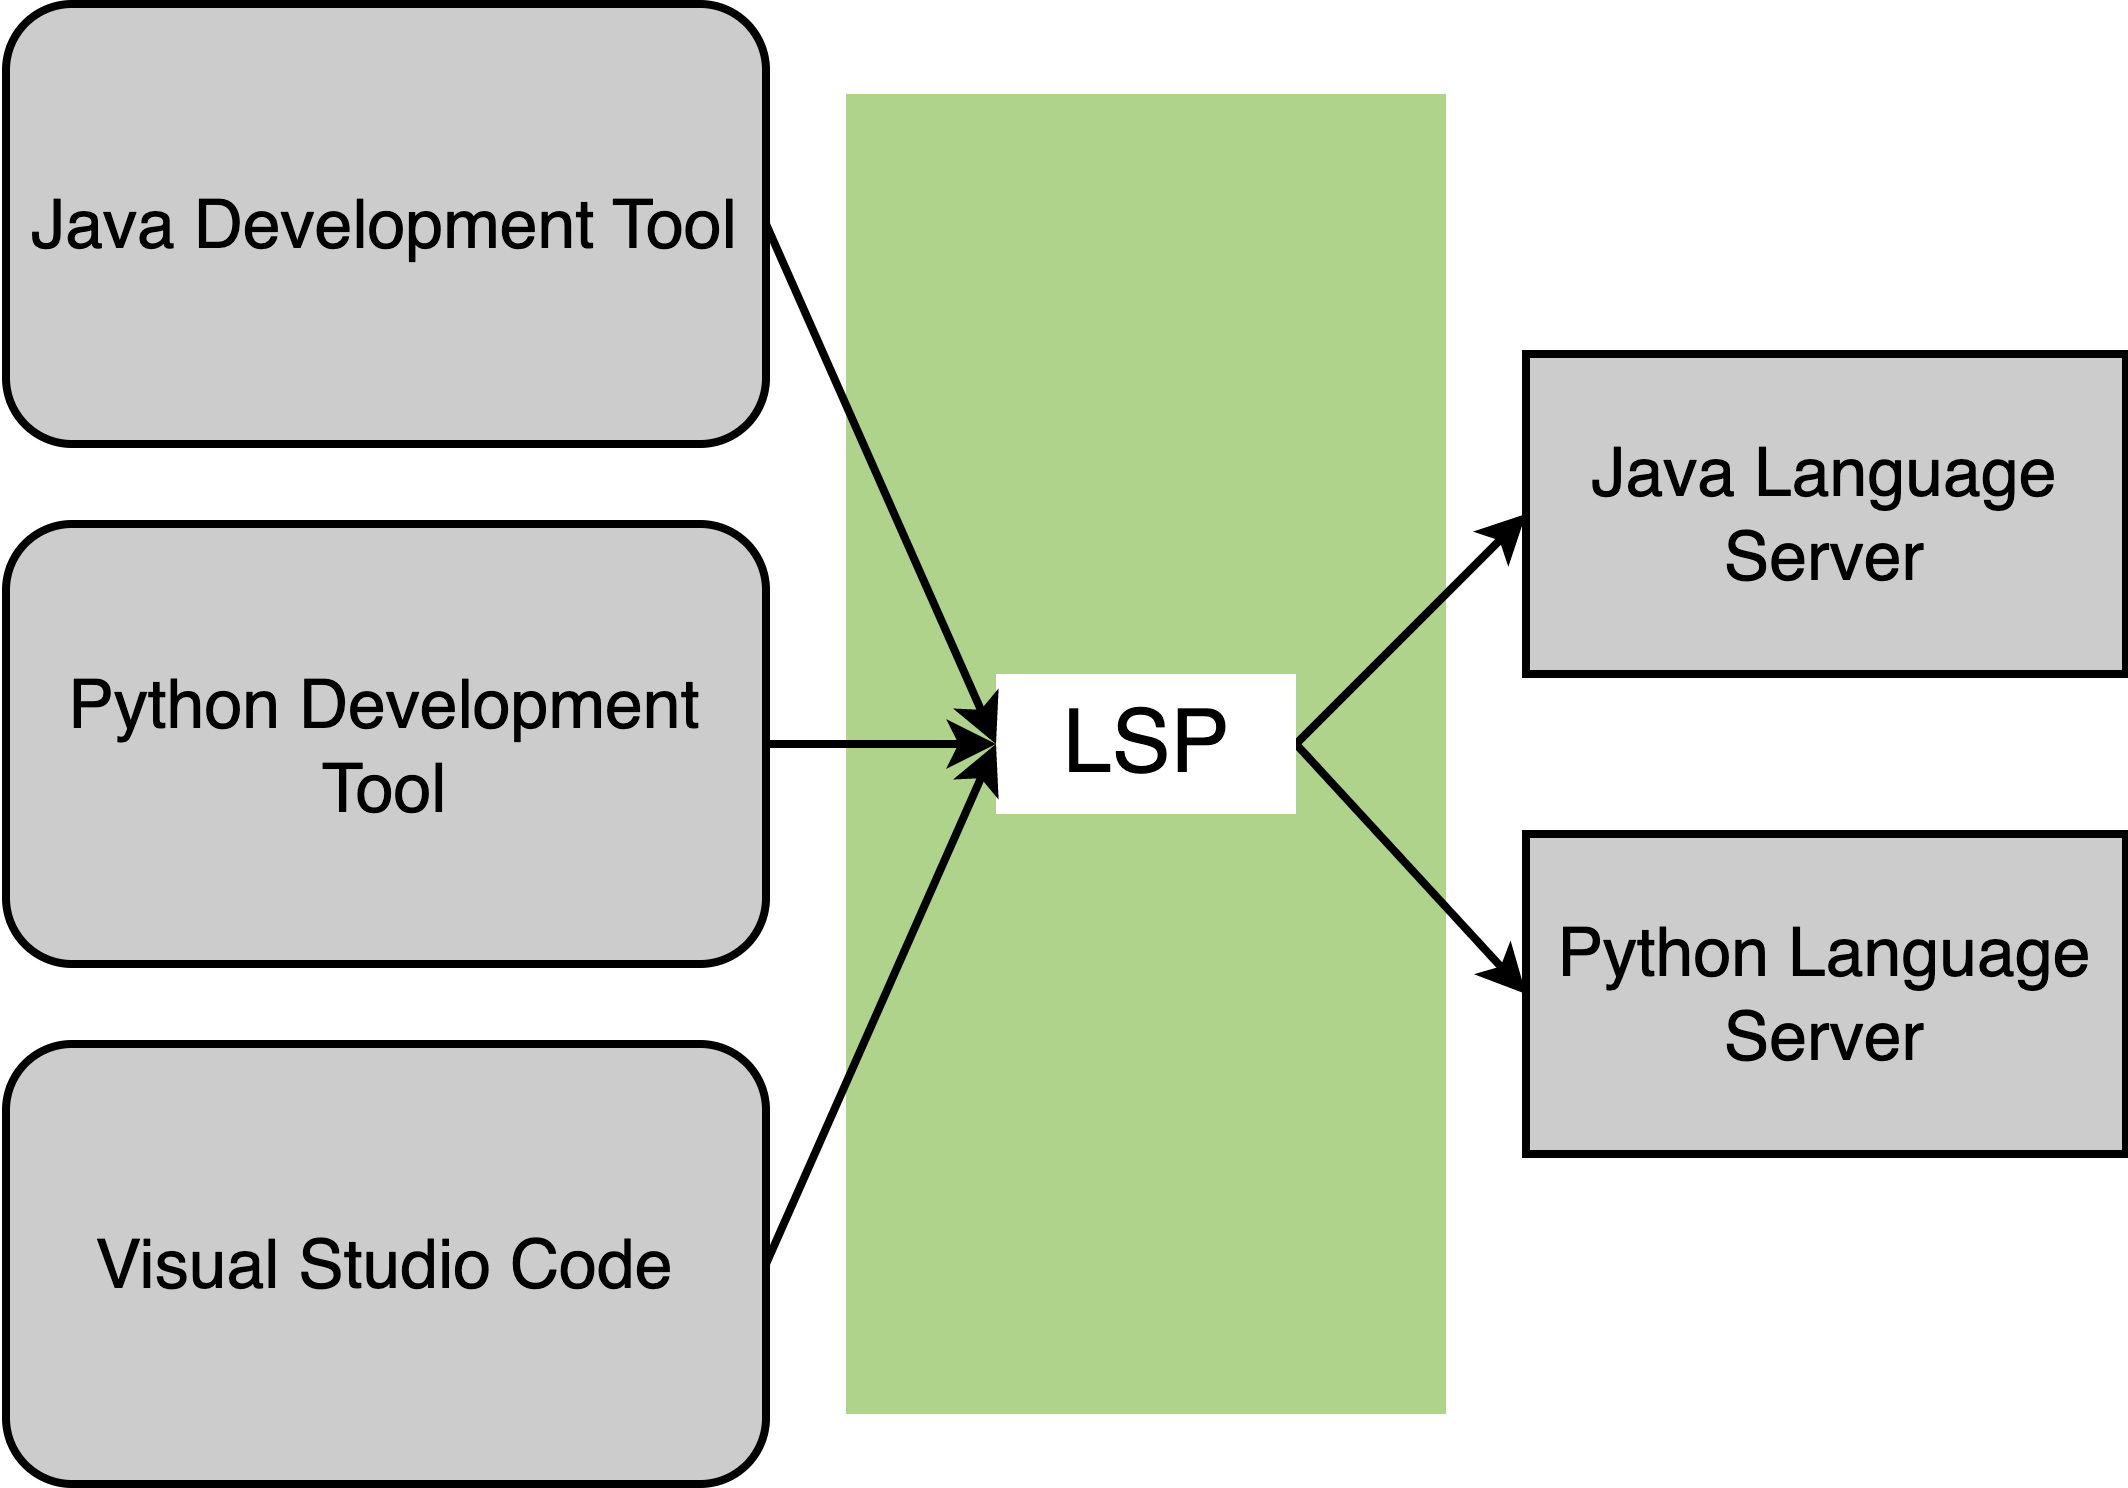
\includegraphics[width=\textwidth]{lsp-theory.png}
            \caption{The Language Server Protocol streamlines the communication between development tools and language servers.}
            \label{fig:lsp-theory}
        \end{center}
    \end{subfigure}
    \caption{Demonatrating the benefit of VS Code's Language Server Protocol.}
    \label{fig:lsp}
\end{figure}

In VS Code extensions, a language server (using LSP) can provide a number of different features for a programming language. By implementing support for the \lstinline{textDocument/hover} request, an exstension could display additional documentation about code when a user hovers their cursor over some text. By implementing support for the \lstinline{widnow/showMessage} request, an extension can display an error message in VS Code's UI when code fails to build. With the \lstinline{textDocument/publishDiagnostics} notification, an extension can validate that a program will run before a user actually tries to run it. For a full list of LSP specificatons, see the documentation \cite{Microsoft_2023i}.

\subsection{Language Servers in Snail Language Support}

In the Snail Language Support extension, we use a language server to validate snail files before runtime, checking for lexer and parser errors. With the extension enabled, VS Code is able to display lexer and parser errors, and highlight the relevant location of the error, before a developer runs the program themselves. This behavior is illustrated in figure \ref{fig:dev-diagnostics}. 

\begin{figure}[t]
    \begin{subfigure}{0.45\textwidth}
        \begin{center}
            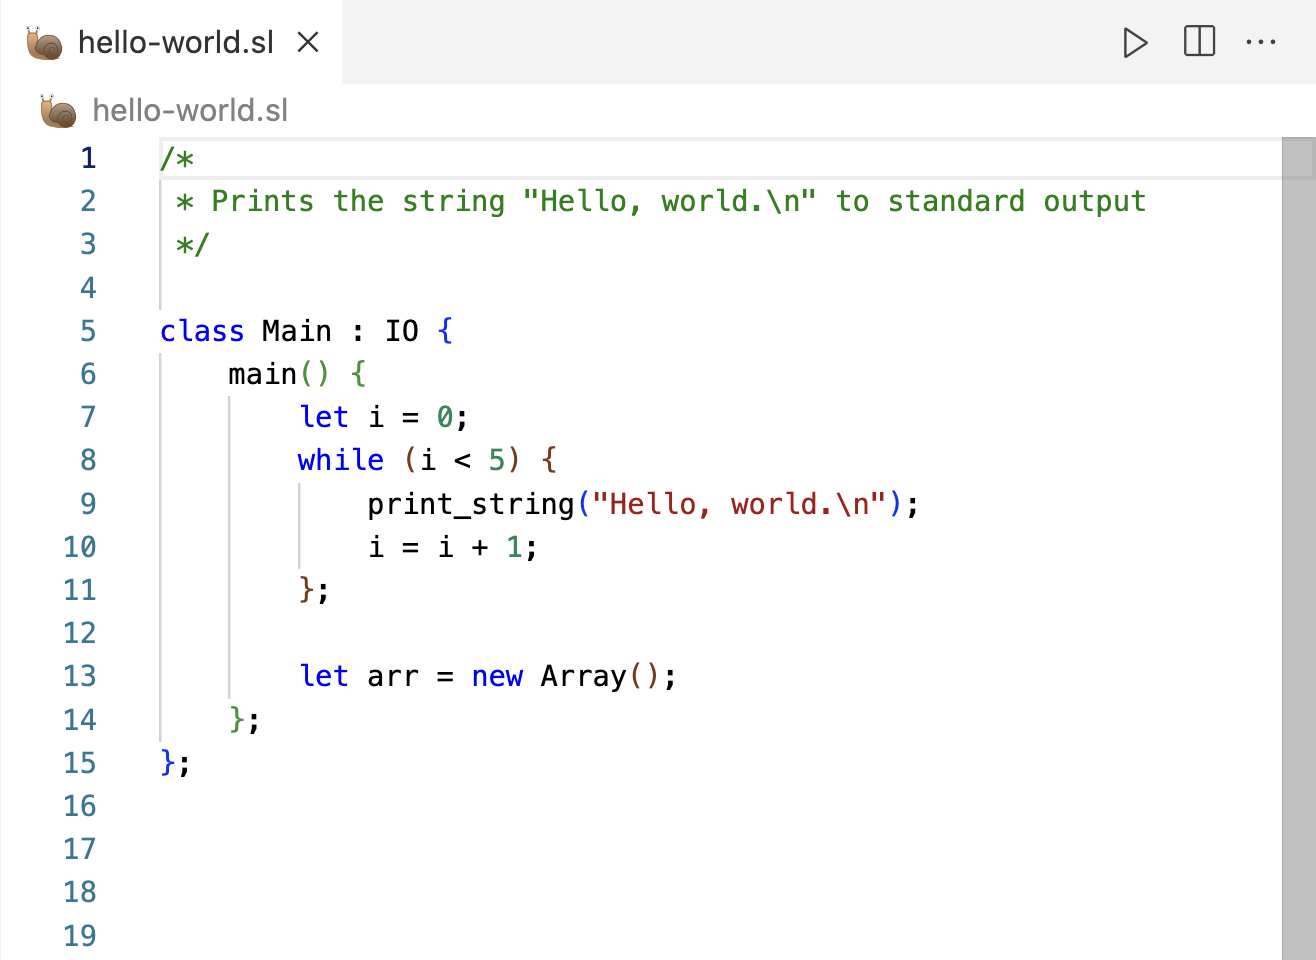
\includegraphics[width=\textwidth]{dev-no-diagnostics-light.png}
            \subcaption{
                \centering
                    Developing snail code without realtime error diagnostics can make it difficult to spot syntax errors.
                }
            \label{fig:dev-no-diagnostics}
        \end{center}
    \end{subfigure}
    \hspace{0.05\textwidth}
    \begin{subfigure}{0.45\textwidth}
        \begin{center}
            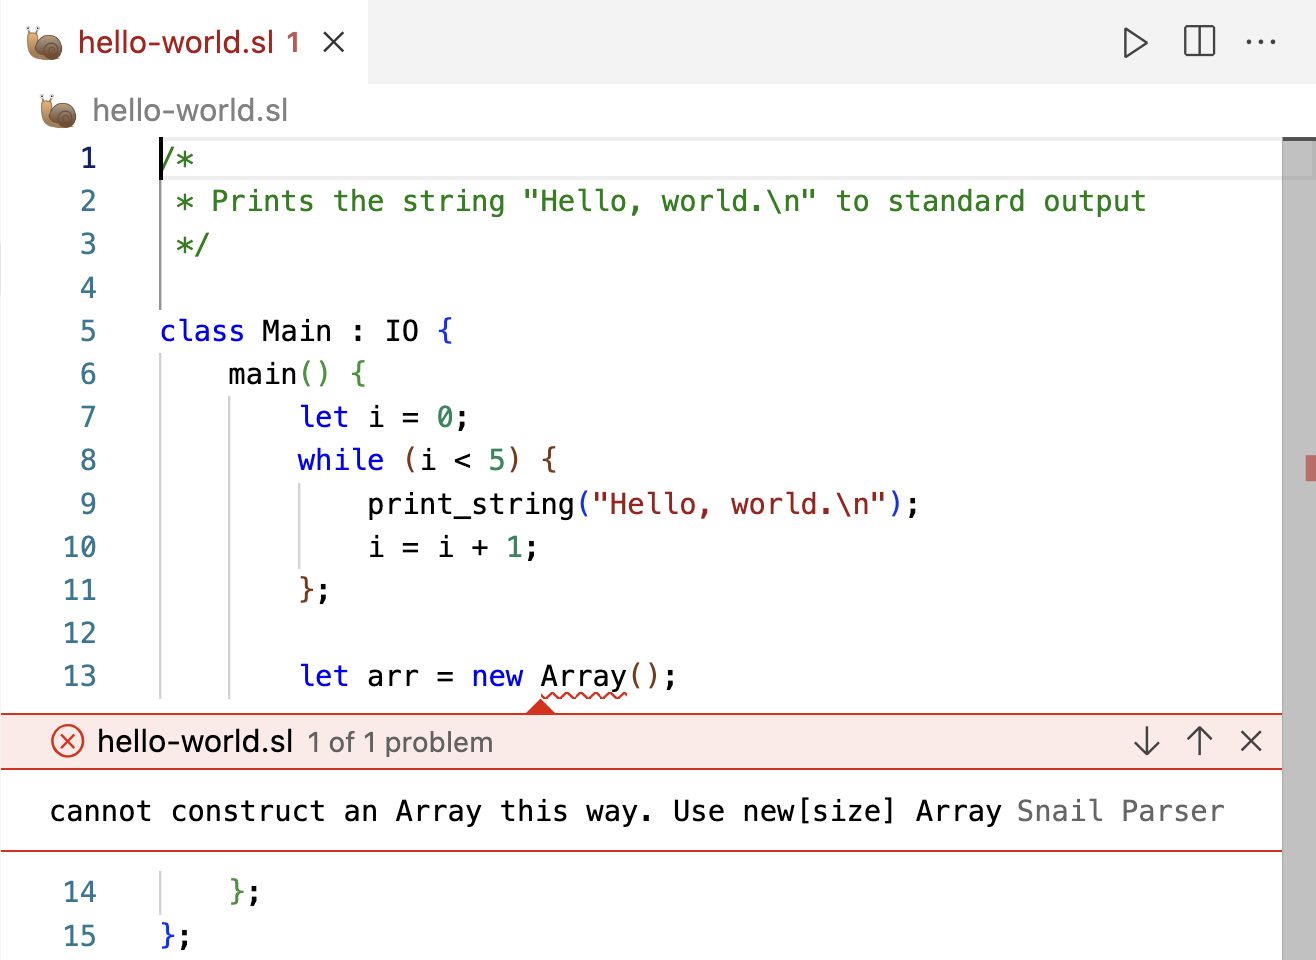
\includegraphics[width=\textwidth]{dev-with-diagnostics-light.png}
            \subcaption{
                \centering
                    With Snail Language Support, a developer can spot easily spot syntax errors and fix them before runtime.
                }
            \label{fig:dev-with-diagnostics}
        \end{center}
    \end{subfigure}
    \caption{
        \centering
            Demonstrating the benefit of realtime error diagnostics provided in Snail Language Support.
        }
    \label{fig:dev-diagnostics}
\end{figure}

\begin{wrapfigure}{R}{0.5\textwidth}
    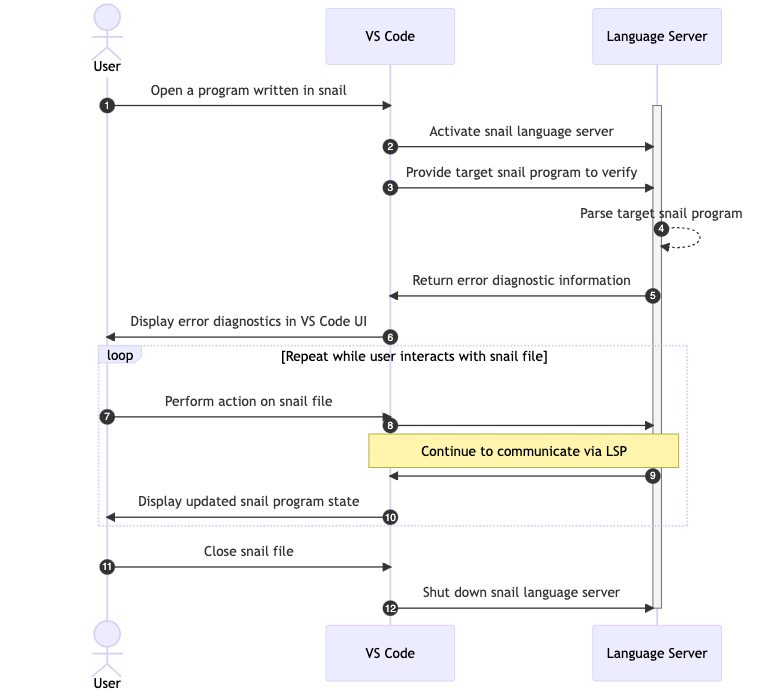
\includegraphics[width=0.5\textwidth]{lsp-sequence.png}
    \caption{
        \centering
            Modelling the interactions between a developer, a VS Code client, and snail language server while a developer opens and modifies a snail file.
    }
    \label{fig:lsp-sequence}
\end{wrapfigure}

To do this, Snail Language Support uses a snail language server. The majority of this language server is implemented in TypeScript in the \lstinline{server.ts} file, which can be found in appendix \ref{app:server-ts}. This file responds to connections from a VS Code client and handles a few important LSP requests such as \lstinline{Initialize} events and \lstinline{DidChangeTextDocument} notifications.

The snail-specific features are provided by modifying the snail interpreter to act as a language server. By passing a \lstinline{-s} or \lstinline{--server} flag while executing a snail file (i.e. \lstinline{snail -s hello-world.sl}), the snail interpreter outputs relevant error diagnostics including program exit status, error source, and error location.\footnote{Further modifying the snail interpreter to handle a variety of potential language server requests (not just requests for error diagnostics) is a great area for future work.} The \lstinline{server.ts} file handles this output and provides it to the VS Code client in the LSP format.

A high-level sequence of interactions between a developer, VS Code client, and snail language server is documented in figure \ref{fig:lsp-sequence}. First, a user opens a program written in snail (1). When the VS Code client detects this activity, it launches a snail language server (2). Next, the VS Code client provides the snail program to verify (3) and the language server executes the snail program, using the aforementioned \lstinline{snail -s} option (4). The snail language server returns the error diagnostics to the VS Code client (5) and the client displays these diagnostics to the developer (6). While the developer further modifies the snail file, the VS Code client and snail language server continue to communicate via LSP (7-10). When a developer is finished, they can close the snail file (11) and the VS Code client shuts down the snail language server (12). 


\section{Debug Adapter Protocol}

Snail Language Support is also structured to support the implementation of a debugger for snail. To do this, Snail Language Support defines a debug adapter that uses VS Code's Debug Adapter Protocol (DAP). In this section, we will discuss what the DAP is and how Snail Language Support uses it.

\subsection{What is the Debug Adapter Protocol?}

Debugging tools are an integral part of the software development process. Modern debuggers are often implemented with a user-friendly UI to help developers debug their programs \cite{Microsoft_2022b,Matloff_Salzman_2008,Sinha_2017}. Many of these debuggers are built intertwined with their corresponding code editor's UI, which can vary from code editor to code editor. As a result, valuable debugging-logic is intermingled with code-editor-specific UI logic. This makes it nearly impossible to implement a debugger that is capable of communicating with different code editors \cite{Microsoft_2021a}. This problem is illustrated in figure \ref{fig:no-dap-theory}.

Instead of asking a development tool to interface directly with a debugger, suppose a development tool interfaces with a debug adapter that translates a development tool's requests and sends them to a language-specific (but tool-agnostic) debugger. If the communication between the development tool and debug adapter is standardized, a language-specific debug adapter can be reused across multiple development tools. 

VS Code's Debug Adapter Protocol (DAP) standardizes the communication between a development tool and debug adapter. As shown in figure \ref{fig:dap-theory}, this allows language-specific debuggers and debug adapters to be reused for multiple development tools.

\begin{figure}[h]
    \begin{subfigure}[c][][c]{0.45\textwidth}
        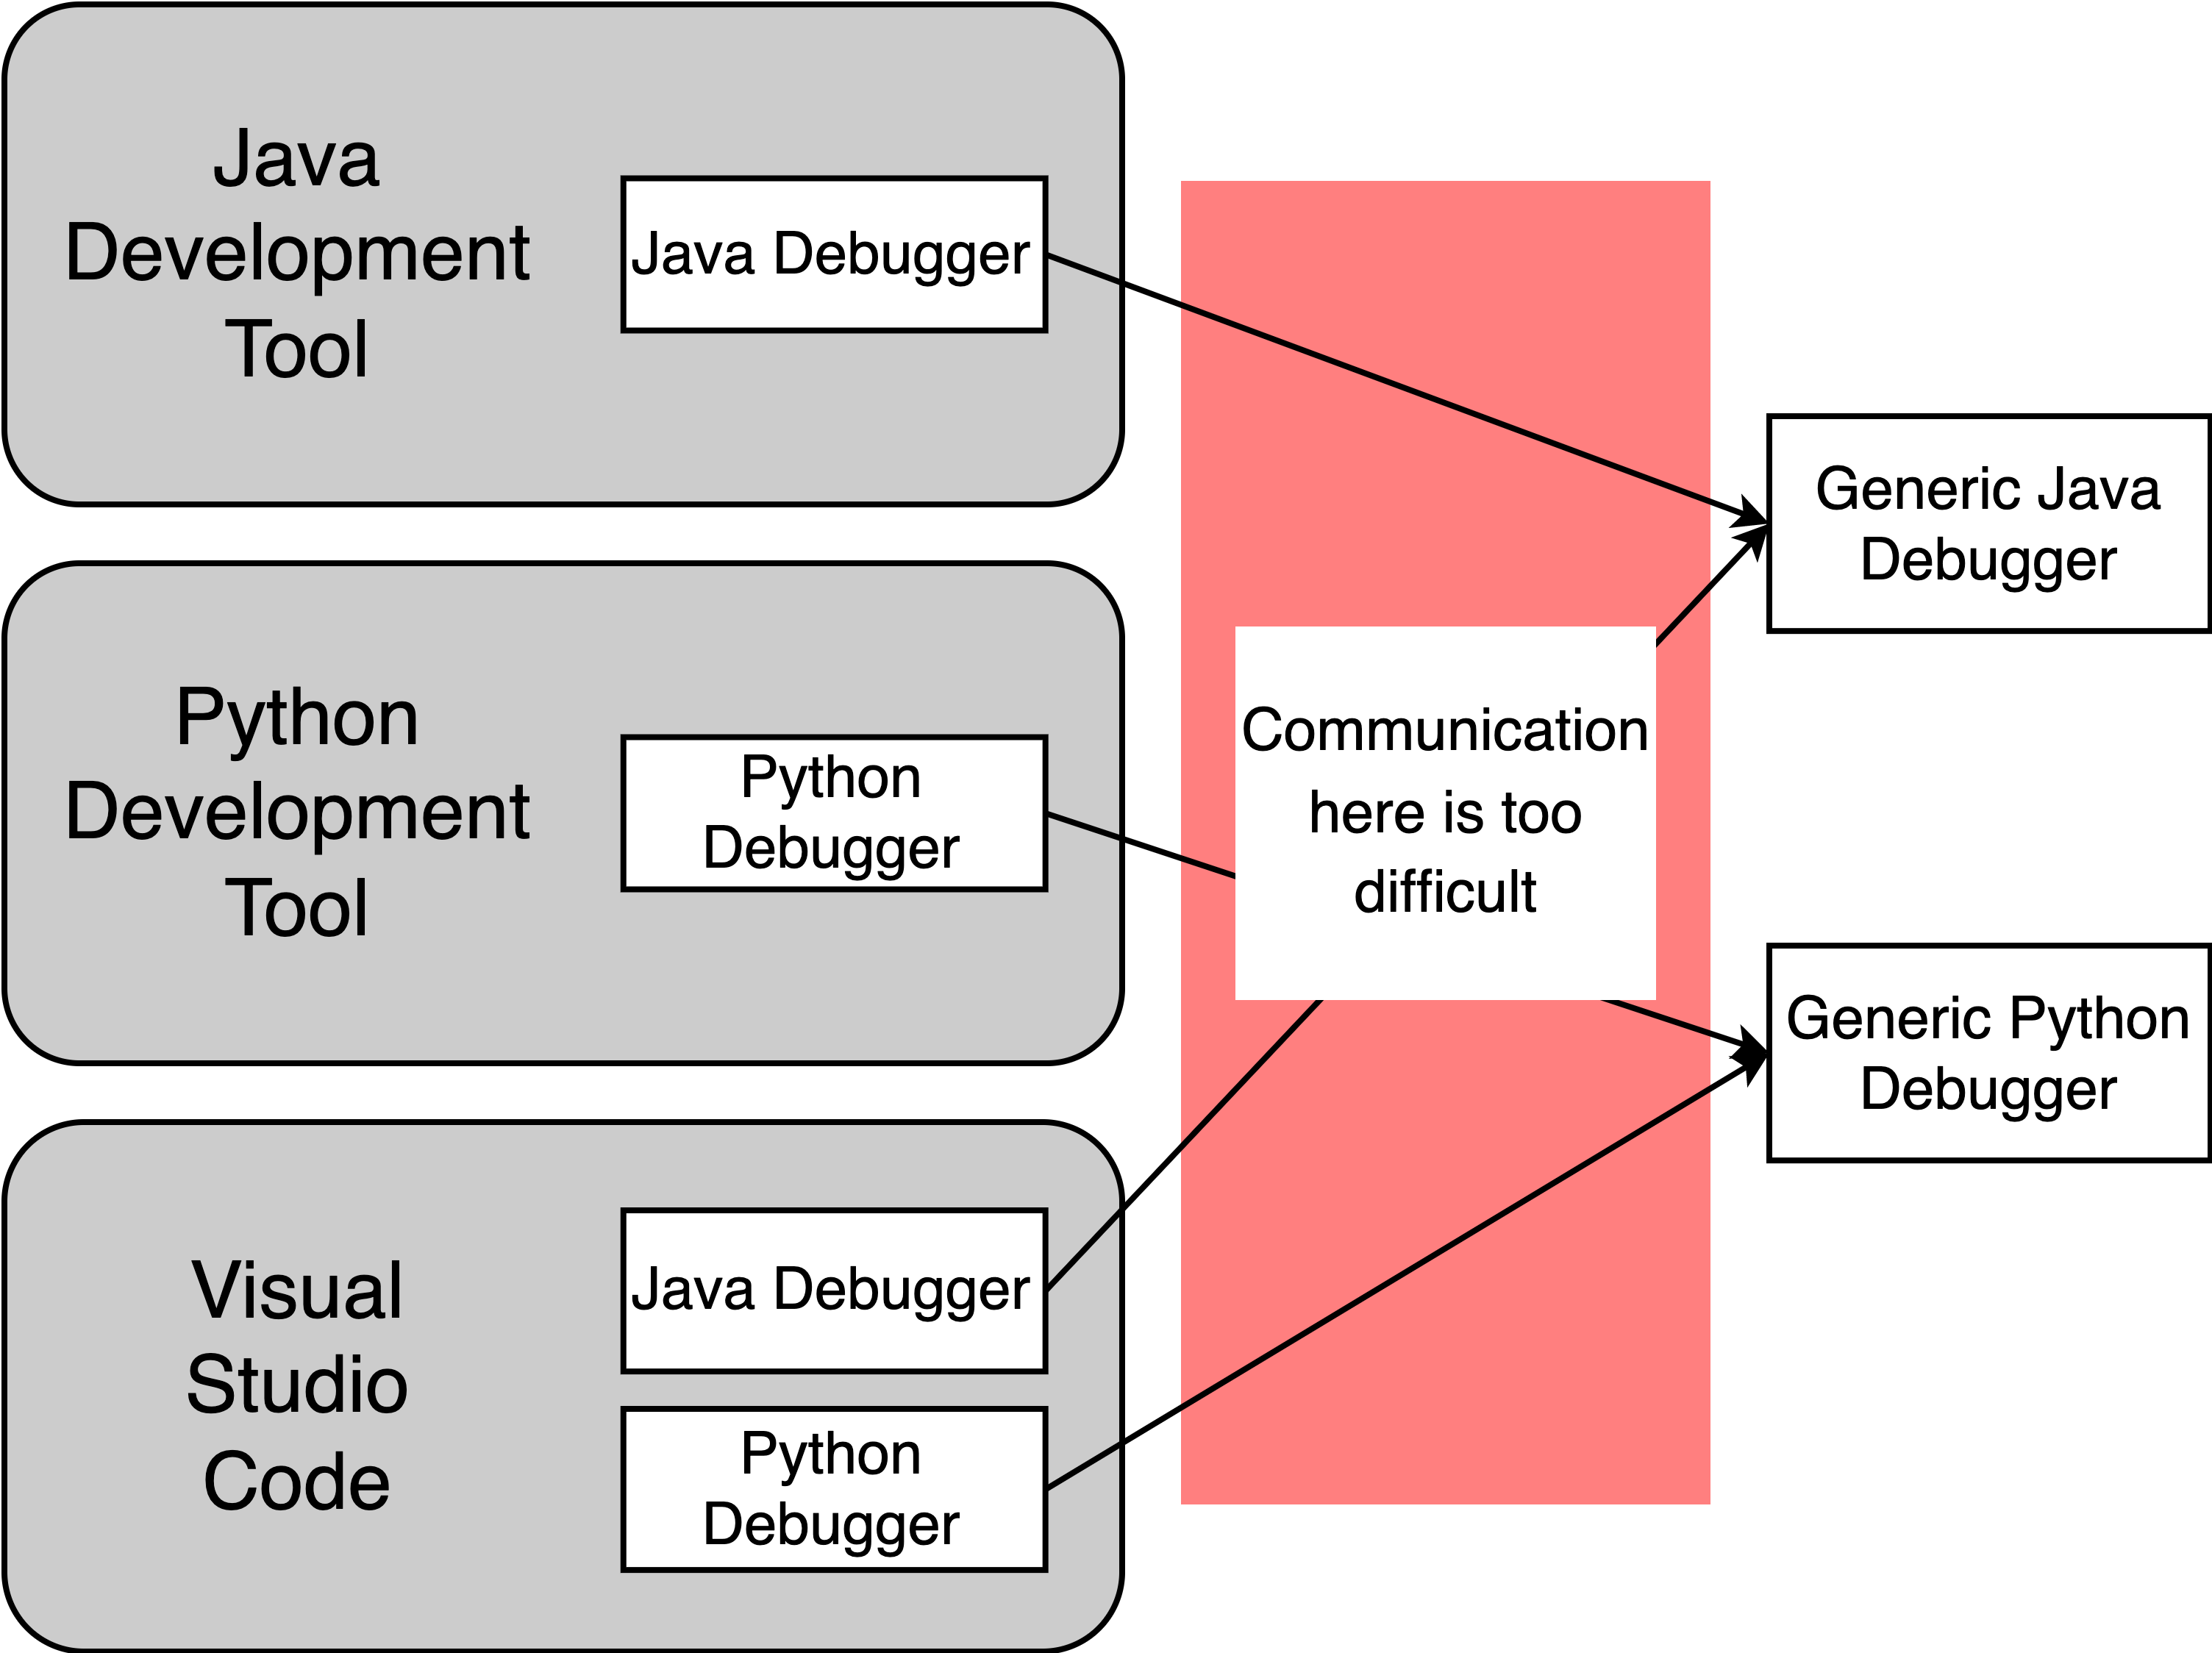
\includegraphics[width=\textwidth]{no-dap-theory.png}
        \caption{Communication between a generic debugger and a development tool is incredibly complicated.}
        \label{fig:no-dap-theory}
    \end{subfigure}
    \hspace{0.05\textwidth}
    \begin{subfigure}[c][][c]{0.45\textwidth}
        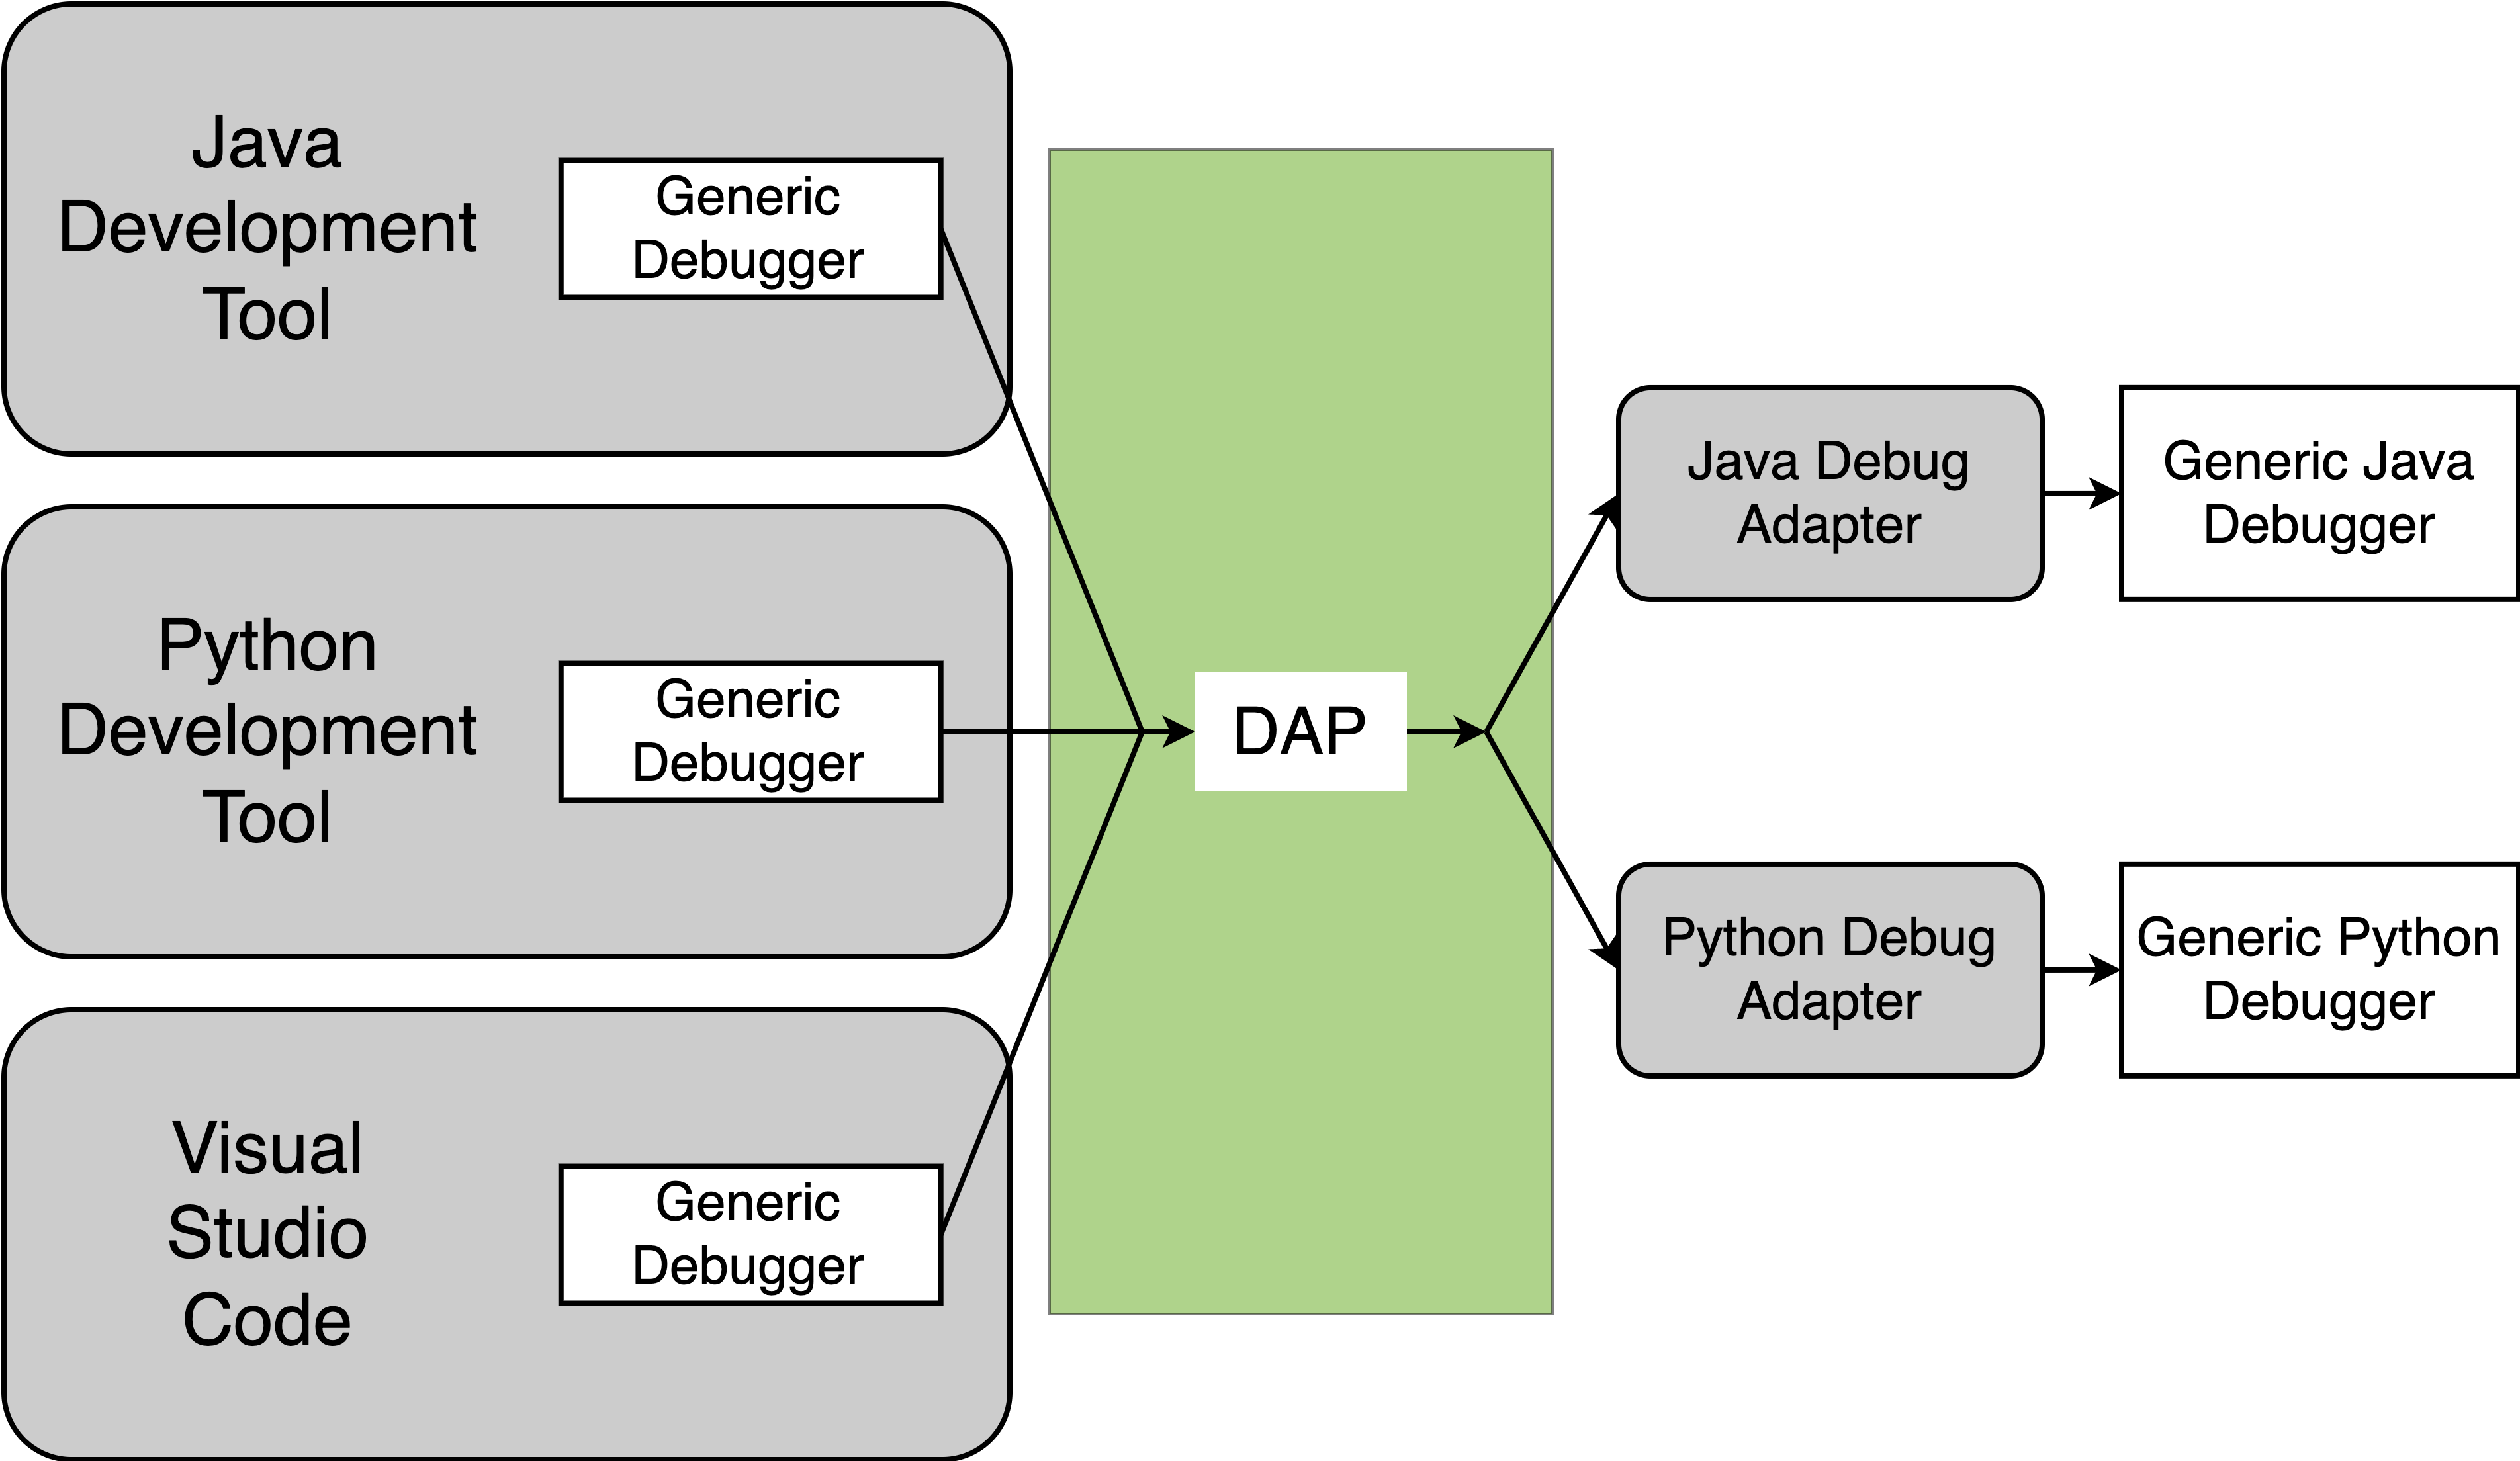
\includegraphics[width=\textwidth]{dap-theory.png}
        \caption{With the Debug Adapter Protocol, a development tool can easily communicate with a generic langauge-specific debugger.}
        \label{fig:dap-theory}
    \end{subfigure}
    \caption{Illustrating the benefit of the Debug Adapter Protocol in aiding development tool and debugger communication.}
    \label{fig:dap}
\end{figure}

VS Code's DAP relies on requests and responses very similarly to the LSP \cite{Microsoft_2021b}. A request is a message that a development tool sends to a debug adapter, asking the debugger to perform some debugging task. The debug adapter communicates with the language-specific debugger to perform this operation and sends a corresponding response message to the development tool. The debug adapter \textbf{must} send a corresponding response after recieving a request, even if the response is an empty message. The DAP also defines reverse requests, which function the same as regular requests except that they are sent from the debug adapter to the development tool.

VS Code's DAP also allows a debug adapter to send the development tool events. This allows the debug adapter to update the development tool on a debugging session's state. For example, a debug adapter can send the development tool a \lstinline{Stopped} event when program execution has stopped due to a breakpoint, step request completion, or expression evaluation completion. 

\subsection{Debug Adapter Protocol in Snail Language Support}

Snail Language Support does not currently provide a debugger for the snail language. However, the extension is structured to support a snail debugger in the future. 

\begin{itemize}
    \item defining a debug adapter for the extension
    \item defining a debug adapter inside of snail
    \begin{itemize}
        \item reasonML
        \item ocaml-dap
        \item lwt
    \end{itemize}
    \item initialization process of that debug adapter (incl. diagram)
    \item appendix of commands to implement in the future (incl. diagram)
\end{itemize}

\section{Good Practices in Software Development}

\subsection{Version Control}

\subsection{Documentation}

\section{Conclusions}

%== BIBLIOGRAPHY ==%
\newpage

\bibliography{refs.bib}
\bibliographystyle{plain}

%== APPENDICES ==%
\newpage

\begin{appendices}

\section{Snail Language Support extension.ts}

    The following is the \lstinline{extension.ts} file from Snail Language Support.

    TODO mesh TypeScript and Json formats to look more uniform

    \lstinputlisting[language=TypeScript]{
        /Users/charlesreinhardt/Git/snail-language-support/client/src/extension.ts
    }
    \label{app:extension-ts}

\newpage
\section{Snail Language Support package.json}

    The following is the \lstinline{package.json} file from Snail Language Support.
    \lstinputlisting[language=json]{
        % this absolute path must be different when building on different machines
        /Users/charlesreinhardt/Git/snail-language-support/package.json
    }
    \label{app:package-json}

\newpage
\section{Snail Language Support language-configuration.json}

    The following is the \lstinline{language-configuration.json} file from Snail Language Support.
    \lstinputlisting[language=json]{
        /Users/charlesreinhardt/Git/snail-language-support/configurations/language-configuration.json
    }
    \label{app:language-configuration}

\newpage
\section{Snail Language Support snippets.json}

    The following is the \lstinline{snippets.json} file from Snail Language Support.
    \lstinputlisting[language=json]{
        /Users/charlesreinhardt/Git/snail-language-support/snippets/snippets.json
    }
    \label{app:snippets-json}

\newpage
\section{Snail Language Support TextMate Grammar}

    The following is the \lstinline{snail.tmLanguage.json} file from Snail Language Support.
    \lstinputlisting[language=json]{
        /Users/charlesreinhardt/Git/snail-language-support/syntaxes/snail.tmLanguage.json
    }
    \label{app:snail-tmLanguage}

\newpage
\section{Snail Language Support server.ts}

    The following is the \lstinline{server.ts} file from Snail Language Support.
    \lstinputlisting[language=TypeScript]{
        /Users/charlesreinhardt/Git/snail-language-support/client/src/server.ts
    }
    \label{app:server-ts}

\end{appendices}

\end{document}